% Created 2020-03-19 Thu 15:02
% Intended LaTeX compiler: pdflatex
\documentclass[11pt]{article}
\usepackage[utf8x]{inputenc}
\usepackage[T1]{fontenc}
\usepackage{graphicx}
\usepackage{grffile}
\usepackage{longtable}
\usepackage{wrapfig}
\usepackage{rotating}
\usepackage[normalem]{ulem}
\usepackage{amsmath}
\usepackage{textcomp}
\usepackage{amssymb}
\usepackage{capt-of}
\usepackage{hyperref}
\usepackage{minted}
\author{Jakub Zárybnický (xzaryb00@stud.fit.vutbr.cz)}
\date{\today}
\title{Genome Browser}
\hypersetup{
 pdfauthor={Jakub Zárybnický (xzaryb00@stud.fit.vutbr.cz)},
 pdftitle={Genome Browser},
 pdfkeywords={},
 pdfsubject={},
 pdfcreator={Emacs 26.3 (Org mode 9.1.9)}, 
 pdflang={Czech}}
\begin{document}

\maketitle

\section{Úkol 1}
\label{sec:orgfe93d07}
Zjistěte, zda obsahuje gen BRCA1 u myši SNP elementy. Pokud ano, znázorněte v
Genome Browseru synonymní SNP modrou barvou a nesynonymní červenou
barvou.

\textbf{Postup:}
\begin{enumerate}
\item Otevřete si prohlížeč se stránkou UCSC Genome Browser
(\url{http://genome.ucsc.edu/}) a přejděte do části pro prohlížení genomů (záložka
Genomes).
\item Zvolte group: \textbf{Mammal}, genome: \textbf{Mouse}, assembly: \textbf{July 2007}.
\item Do textového pole vložte název \textbf{Brca1} a stiskněte tlačítko \textbf{Submit}.
\item V seznamu zobrazených výsledků (sekce UCSC Genes) si vyberte ten, který je
uveden jako první. Kliknutím na tuto položku v hlavním okně Genome Browseru
se dozvíte podrobné informace o tomto genu včetně struktury jeho
proteinu. Vraťte se zpět.
\item Přejděte níže do sekce obsahující seznam stop a jejich konfiguraci.  Klikněte
na odkaz \textbf{SNPs (128)} ze skupiny \textbf{Variation and Repeats}. V této části si můžete
prohlédnout aktuální nastavení pro zobrazení této stopy včetně dalších
možností její vizualizace.
\item V sekci \textbf{Coloring Options} vyberte modrou barvu pro \textbf{Coding - Synonymous} a
červenou barvu pro \textbf{Coding - Non-Synonymous}. Potvrďte tlačítkem \textbf{Submit}.
\item V grafickém prohlížeči prozkoumejte upravenou stopu \textbf{SNPs (128)}.  Měli by jste
nyní přehledně vidět výskyty synonymních i nesynonymních mutací genu \textbf{Brca1}.
\item Kliknutím na libovolnou položku stopy \textbf{SNPs (128)} si můžete prohlédnout
podrobnější informace o příslušné mutaci.
\end{enumerate}

\textbf{=> Nesynonymních SNP jsem napočítal 13, synonymních 15}

\section{Úkol 2}
\label{sec:orge1f197e}
S využitím Table Browser-u získejte seznam SNP elementů pro gen Clock u člověka.

\textbf{Postup:}
\begin{enumerate}
\item Otevřete si prohlížeč se stránkou UCSC Genome Browser
(\url{http://genome.ucsc.edu/}) a přejděte do části pro práci s tabulkami (záložka
Tables).
\item Zvolte clade: \textbf{Mammal}, genome: \textbf{Human}, assembly: \textbf{Feb. 2009}.
\item Vyberte skupinu \textbf{Variation}, stopu: \textbf{Common SNPs(138)} a tabulku \textbf{snp138Common}.
\item Do textového pole pro pozici vložte název \textbf{Clock} a stiskněte tlačítko \textbf{lookup}.
\item Zobrazí se vám seznam výsledků se záznamem \textbf{Clock}. Vyberte odkaz \textbf{Homo sapiens
clock circadian regulator (CLOCK), transcript variant 1, mRNA} na pozici
\textbf{chr4:56294068-56412099}.
\item Ponechte nastavení filtru a průsečíku nevyplněné.
\item Jako \textbf{Output Format} vyberte \textbf{selected fields from primary and related
tables}. Stiskněte tlačítko \textbf{get output}.
\item Ve výsledné nabídce zaškrtněte políčka: \textbf{chrom, chromStart, chromEnd, name,
strand, observed} a \textbf{func}. Stiskněte tlačítko \textbf{get output}.
\item Zobrazí se vám výsledný seznam položek, které si můžete zkopírovat nebo
uložit pro další studium. Kolik jste našli položek?
\end{enumerate}

\textbf{=> 550 řádků výstupu (1 řádek hlavičky, 549 SNP)}

\section{Úkol 3}
\label{sec:orgb92bbd8}
S využitím Table Browser-u získejte seznam známých genů člověka vyskytujících se
na konci chromozomu 22, ve kterých se nacházejí CpG ostrůvky (CpG
islands). Získejte sekvence těchto genů ve formátu FASTA.

\textbf{Postup:}

\begin{enumerate}
\item Otevřete si prohlížeč se stránkou UCSC Genome Browser
(\url{http://genome.ucsc.edu/}) a přejděte do části pro práci s tabulkami (záložka
Tables).
\item Zvolte clade: \textbf{Mammal}, genome: \textbf{Human}, assembly: \textbf{Feb. 2009}.
\item Vyberte skupinu \textbf{Genes and Gene Predictions Tracks}, stopu: \textbf{UCSC Genes} a
tabulku \textbf{knownGene}.
\item Do textového pole pro pozici vložte název \textbf{chr22} a stiskněte tlačítko
\textbf{lookup}. Počáteční pozici upravte na \textbf{40.000.000}.
\item Stiskněte tlačítko \textbf{intersection}.
\item Vyberte skupinu \textbf{Regulation} a stopu \textbf{CpG Islands}. Ostatní volby ponechte v
původním nastavení a stiskněte tlačítko \textbf{submit}.
\item Jako \textbf{Output Format} vyberte \textbf{sequence}. Stiskněte tlačítko \textbf{get output}.
\item Ve výsledné nabídce vyberte \textbf{genomic}. Stiskněte tlačítko \textbf{submit}.
\item Ujistěte se, že volby \textbf{5' UTR Exons, CDS Exons, 3' UTR Exons} jsou zaškrtnuty
a volba \textbf{Introns} odškrtnuta. Zvolte \textbf{One FASTA record per region} a ponechte
ostatní volby v původním nastavení. Stiskněte tlačítko \textbf{Get Sequence}.
\item Zobrazí se vám výsledný seznam položek, které si můžete zkopírovat nebo
uložit pro další studium. Kolik jste našli položek?
\end{enumerate}

\textbf{=> 4021 fasta záznamů}

\section{Úkol 4}
\label{sec:org84ea6a1}
Prostudujte si návod na vytváření vlastních stop v Genome Browser-u a vytvořte
vlastní stopu, která bude znázorňovat geny člověka na chromozomu 22, jejichž
délka je větší než 100k bází.

\textbf{Postup:}
\begin{enumerate}
\item Otevřete si prohlížeč se stránkou UCSC Genome Browser
(\url{http://genome.ucsc.edu/}) a prostudujte si návod na vytváření vlastních stop
(záložka \textbf{Help}).
\item Přejděte do části pro práci s tabulkami (záložka \textbf{Tables}).
\item Zvolte clade: \textbf{Mammal}, genome: \textbf{Human}, assembly: \textbf{Feb. 2009}.
\item Vyberte skupinu \textbf{Genes and Gene Predictions Tracks}, stopu: \textbf{UCSC Genes} a
tabulku \textbf{knownGene}.
\item Do textového pole pro pozici vložte název \textbf{chr22} a stiskněte tlačítko
\textbf{lookup}. Počáteční pozici upravte na \textbf{40.000.000}.
\item Volby \textbf{filter} a \textbf{intersection} ponechte prázdné.
\item Jako \textbf{Output Format} vyberte \textbf{BED - browser extensible data}. Do položky \textbf{output
file} vložte název výsledného souboru. Stiskněte tlačítko \textbf{get output}.
\item Ve výsledné nabídce zvolte volbu \textbf{Whole Gene}. Stiskněte tlačítko \textbf{get BED}.
\item Vytvořte si jednoduchý skript (Python, Perl, AWK, \ldots{}), který přečte soubor
ve formátu \textbf{BED} a vypíše pouze ty geny, jejichž délka je větší než 100k
bází. Výstup skriptu opět uložte do souboru ve formátu \textbf{BED}.
\item Vytvořený soubor vložte jako novou stopu do Geonome Browseru.
\end{enumerate}

\begin{center}
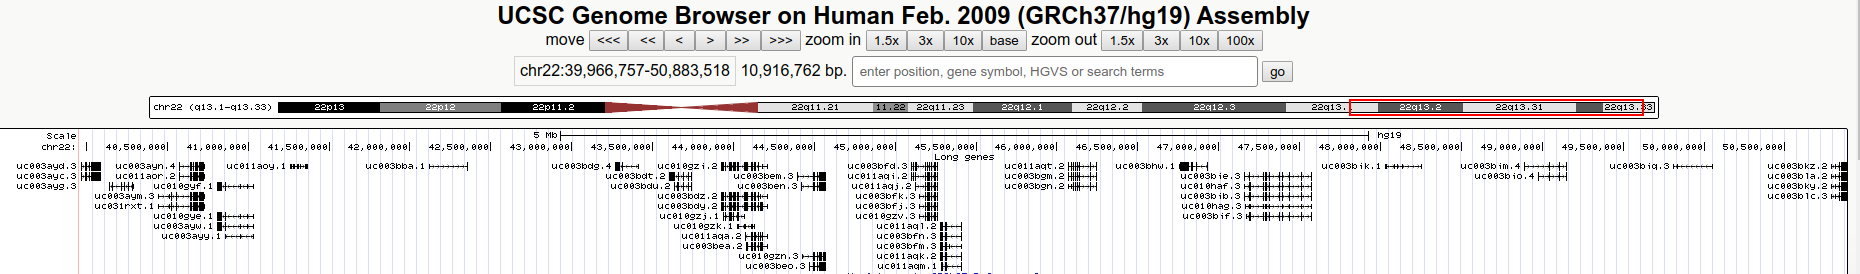
\includegraphics[width=1.2\linewidth]{./bif-3-custom.png}
\end{center}

\section{Vysvětlivky}
\label{sec:orgd6de9e8}
\begin{itemize}
\item \textbf{SNP (Single-nucleotide polymorphism)}: označuje takový nukleotid v genomu,
který se liší mezi jednotlivými členy určitého druhu nebo mezi párovými
chromozomy příslušného jedince.
\item \textbf{Synonymní mutace}: mutace kodonu, která nezpůsobí změnu aminokyseliny
výsledného proteinu.
\item \textbf{Nesynonymní mutace}: mutace kodonu, která způsobí změnu aminokyseliny
výsledného proteinu.
\item \textbf{BRCA1}: jedná se o gen, který pomáhá opravovat poškozenou DNA v buňkách
prsu. Pokud je poškozen zvyšuje se riziko rakoviny prsu.  Zdroje: \href{http://en.wikipedia.org/wiki/BRCA1}{wiki}
\item \textbf{CLOCK}: jedná se o gen, který kóduje protein související s režimem spánku. Jeho
mutace mohou vést k poruchám spánku a k bipolárním poruchám. Zdroje: \href{http://en.wikipedia.org/wiki/CLOCK}{wiki},
\href{http://www.youtube.com/watch?v=XzcdZ-MAyus}{youtube video}.
\item \textbf{CpG ostrůvek}: jedná se o oblasti genomu, ve kterých je vysoká koncentrace CpG
bází (kde p označuje fosfátovou vazbu).
\end{itemize}
\end{document}